% HydroPin - technical report (TSYP 14 AOTN, Phase 3), first draft.
% Template: IEEE Conference (IEEEtran, two columns). On Overleaf: New Project -> Upload Project ->
% this folder as a .zip, or open the "IEEE Conference Template" and replace its main.tex.
% Every place that waits for the real bench campaign is marked \TODO{...} (red in the PDF).
\documentclass[conference]{IEEEtran}
\IEEEoverridecommandlockouts
\usepackage{cite}
\usepackage{amsmath,amssymb,amsfonts}
\usepackage{graphicx}
\usepackage{textcomp}
\usepackage{xcolor}
\usepackage{booktabs}
\usepackage{multirow}
\usepackage{url}
\graphicspath{{figures/}}
\newcommand{\TODO}[1]{\textcolor{red}{[TODO: #1]}}
\newcommand{\SIM}{\textsc{sim}}
\def\BibTeX{{\rm B\kern-.05em{\sc i\kern-.025em b}\kern-.08em
    T\kern-.1667em\lower.7ex\hbox{E}\kern-.125emX}}

\begin{document}

\title{HydroPin: Detecting, Locating and Confirming Leaks\\in Pressurised Farm Irrigation Networks}

\author{\IEEEauthorblockN{Talel Laarif, Eya Fetni, Kmar Ben Ayed, Houda Jardak, Israa Soudani}
\IEEEauthorblockA{\textit{Team Ceres, INSAT -- National Institute of Applied Science and Technology} \\
\textit{University of Carthage}, Tunis, Tunisia}}

\maketitle

\begin{abstract}
Drip and sprinkler networks lose water through leaks that farmers notice late, if at all.
HydroPin detects, locates and confirms leaks in pressurised PVC/PE irrigation networks. A low-cost
node reads two pressure transmitters and a flow meter. A detector checks the sensors first, then
fuses a flow test with a pressure-subspace method (M2) into a leak probability, the leaking
branch and the volume lost. A live dashboard and phone alerts present the result. We built the
full chain on a laboratory bench and, in simulation, scaled it to a 50~ha drip farm: sensor
placement against kit cost, localisation with M2 and a graph neural network (M1), and a
rule-based drone confirmation flight. A third method (M3) locates leaks from pressure waves by
time reversal. It is validated against closed-form transient results and reaches sub-metre
accuracy on a simulated 150~m pipe. On 160 simulated bench runs the detector finds every medium
and large leak on the right branch in about 9~s with no false alarm. The bench campaign results
are reported in Section~\ref{sec:bench}. Throughout, measured and simulated results are kept
apart.
\end{abstract}

\begin{IEEEkeywords}
leak detection, irrigation, IoT, sensor fusion, digital twin, graph neural network, hydraulic transients, time reversal
\end{IEEEkeywords}

% =====================================================================
\section{Introduction}
Irrigation is the largest water use in Tunisia, and drip networks run for hours with nobody
watching the pipes. A cracked lateral or a broken fitting wastes water and energy until it shows
on the surface. Two pieces of physics shape the problem. \emph{Detecting} a leak is easy: water
escapes, the pump delivers more flow and slides down its curve, and every pressure in the network
drops. \emph{Locating} it is hard: the pressure drop is almost the same everywhere, and only the
small differences between sensors carry the location.

HydroPin follows a detect--localise--pinpoint pipeline:
\begin{itemize}
\item a flow check and pressure-based methods detect the leak;
\item the pressure pattern over a few sensors gives the branch or pipe;
\item pressure waves (M3) and an optional drone flight confirm the exact spot.
\end{itemize}
The method names are used consistently: \textbf{M1} is the graph neural network, \textbf{M2}
the PCA/subspace method and \textbf{M3} the transient (pressure-wave) method.

This report presents the Phase~3 prototype. Its contributions are:
\begin{enumerate}
\item an end-to-end bench chain (sensor node, broker, backend, detector, dashboard, alerts),
  where the same detector code runs live, in scoring and in replays;
\item a simulated 50~ha farm with 2,070 leak scenarios, a sensor-placement tool that trades
  isolation against kit cost, and a comparison of M2, M1 and their fusion;
\item a validated pressure-wave simulator with four leak locators (echo, time reversal,
  matched-field, 1D CNN).
\end{enumerate}
Every simulated result is labelled as such, in the dashboard as in this report
(Table~\ref{tab:real}).

% =====================================================================
\section{System Overview}
Fig.~\ref{fig:chain} shows the software chain.
\begin{itemize}
\item \textbf{Node:} an ESP32 reads the sensors and publishes one JSON message twice a second
  over WiFi to an MQTT broker on the laptop (amqtt, or Mosquitto), with raw ADC counts next to
  the converted values.
\item \textbf{Backend:} a single Python process on a laptop (FastAPI, paho-mqtt, SQLite)
  validates each message against a frozen contract, stores it, runs the detector and streams
  the result to the dashboard over a WebSocket.
\item \textbf{Exports:} recorded runs are exported as replay files and published as a static
  site on GitHub Pages. Judges can replay real runs without the laptop.
\end{itemize}
Leak states follow the blueprint thresholds: below $\tau_1$ the network is \textsc{healthy};
between $\tau_1$ and $\tau_2$ it is \textsc{watch} (the farm-scale trigger for M3); above
$\tau_2$ for $N$ consecutive samples it is \textsc{leak}.

\begin{figure}[t]
\centering
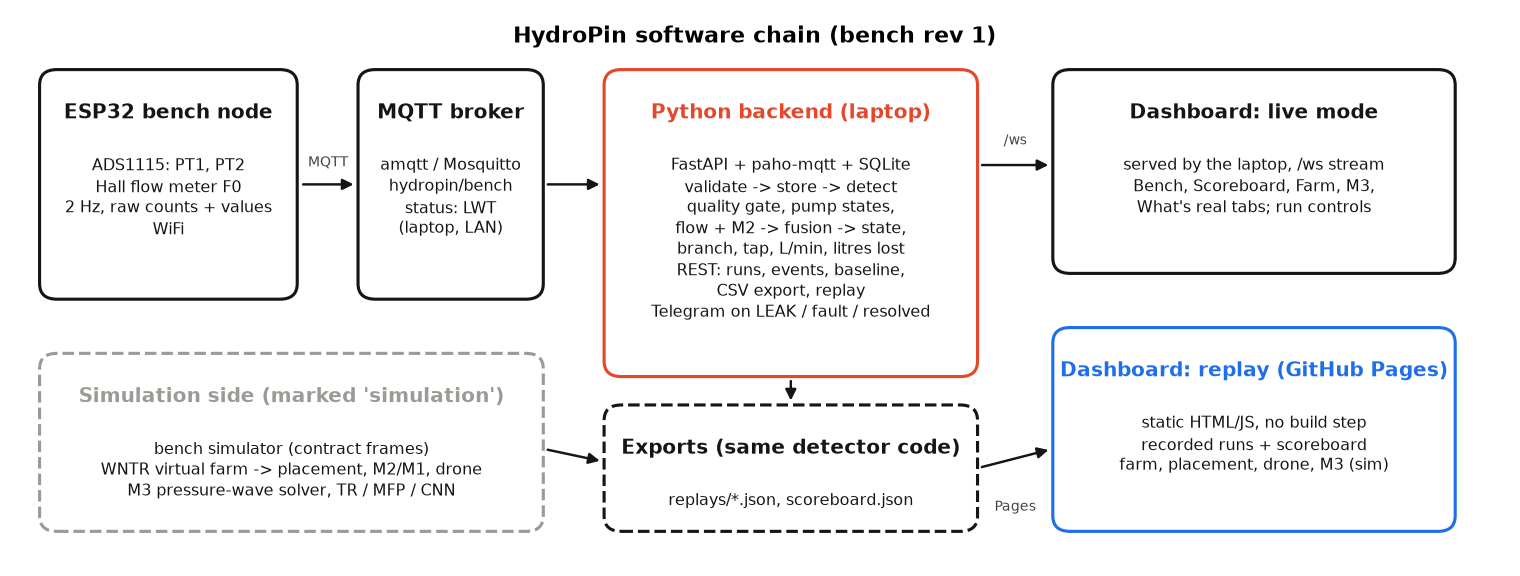
\includegraphics[width=\columnwidth]{software_chain.png}
\caption{HydroPin software chain on the bench. The detector code is shared by the live path,
the scoring and the replay export. Grey: simulation side.}
\label{fig:chain}
\end{figure}

% =====================================================================
\section{Laboratory Bench}
\label{sec:benchhw}
The bench is a closed loop fed from a 20~L bucket by a 12~V pump through 16~mm PE pipe. A
flow meter (F0) sits at the source. A tee splits the loop into two branches:
\begin{itemize}
\item branch A carries tap L1 upstream of pressure transmitter PT1;
\item branch B carries tap L2 upstream and tap L3 downstream of PT2.
\end{itemize}
Opening a tap (or a drilled cap of 0.2--1~mm) creates a controlled leak. Since L2 and L3 share
one sensor, the bench promises the \emph{branch}, not the exact tap. Table~\ref{tab:sensors}
lists the electronics.
\TODO{photo of the bench with sensors and taps labelled; pipe lengths from role~1.}

\begin{table}[t]
\caption{Bench sensing chain (rev.~1)}
\label{tab:sensors}
\centering
\footnotesize
\begin{tabular}{@{}lll@{}}
\toprule
Item & Choice & Conversion / note\\
\midrule
PT1 (branch A) & 0--6 bar, 0--10 V & $p = 0.6\,V_s$ \\
PT2 (branch B) & $-1$--1.6 bar, 0--10 V & $p = -1 + 0.26\,V_s$ \\
Divider & 20k/10k (checked) & $V_s = 3.0\,V_{\mathrm{ADC}}$ \\
ADC & ADS1115, $\pm$4.096 V & 16 bit, 128 SPS \\
F0 & Hall, $\approx$450 pulses/L & 2 s window: 0.1 L/min step\\
Node & ESP32, WiFi + MQTT & 2 Hz, raw counts + values \\
\midrule
Noise $\sigma$$^\ast$ & PT2: 5--7 mbar & PT1: 10--20 mbar, F0: 0.04 L/min\\
Flow $K$ & \multicolumn{2}{l}{\TODO{bucket and stopwatch, two flows}}\\
\midrule
\multicolumn{3}{@{}l@{}}{\scriptsize $^\ast$Preliminary: short-term noise in two bring-up runs (Section~\ref{sec:bench}).}\\
\bottomrule
\end{tabular}
\end{table}

% =====================================================================
\section{Leak Detection on the Bench}
\label{sec:detector}
The detector is one streaming class: each message in, one processed frame out. It never reads
labels or event markers; those are kept for scoring only.

\subsection{Quality gate and pump states}
Bad sensor data must never look like a leak, so the detector checks the sensors before anything
else:
\begin{itemize}
\item a transmitter at its unplugged level for 3~s, out of range, or stuck (identical readings
  for 5~s) raises a \emph{fault};
\item one pressure moving alone while the flow and the other pressure stay flat is a fault, not
  a leak;
\item no data for 3~s gives \textsc{offline}.
\end{itemize}
Faulted sensors are excluded from the methods. After the pump starts, the detector waits 20~s
(\textsc{settling}), then learns a 30~s healthy baseline (\textsc{learning}).

\subsection{Methods}
Signals are smoothed with an exponential moving average ($\tau = 4$~s).

\emph{Flow} compares F0 with its baseline:
\begin{equation}
z_f = \frac{\bar F - F_0}{s_F},\qquad
\ell_f = \mathrm{clip}\big(w_f (z_f - z_0),\,-3,\,5\big).
\end{equation}

\emph{M2} scores the pressure change $\mathbf d = [\Delta P_1, \Delta P_2]^\top$ against the
healthy subspace learned by an SVD of the baseline window. Supply wander moves both pressures
together (common mode), so it is treated as healthy:
\begin{equation}
\Sigma = C + \sigma_p^2 I + \sigma_{cm}^2\,\mathbf u\mathbf u^\top,\qquad
z_2 = \pm\sqrt{\mathbf d^\top \Sigma^{-1}\mathbf d}.
\end{equation}
Here $C$ is the baseline covariance and $\mathbf u$ its first singular vector. The sign of $z_2$
is negative when the pressures rose. M2's log-odds $\ell_2$ follow the same form as $\ell_f$.

\subsection{Fusion, location and size}
The methods that pass the gate are fused as weighted log-odds:
\begin{equation}
p_{\mathrm{leak}} = \sigma\Big(\ell_0 + \ell_f + \max(\ell_2, 0)\Big).
\end{equation}
The floor on $\ell_2$ applies unless the pressures rose. A small leak raises the flow but barely
moves the pressures, so without the floor M2 would veto the flow evidence. The states use
$\tau_1 = 0.5$, $\tau_2 = 0.9$ and $N = 10$ samples (5~s).

The branch comes from the cosine similarity between $\mathbf d$ and a per-tap fingerprint
(prior: L1 drops PT1 about twice as much as PT2; L2 and L3 drop PT2 more), turned into per-tap
probabilities by a softmax ($\kappa = 8$). The leak flow is F0 minus its baseline, and the
volume lost is its integral since detection.

\subsection{Pre-campaign validation in simulation}
A bench simulator emits messages in the exact contract format. It models the base flow
(1.5~L/min at 1.0~bar), tap-specific pressure drops, slow supply wander, sensor noise and the
0.1~L/min flow quantisation. It also covers sensor ripple, dropouts, a WiFi gap, a pump restart
and an unplugged PT1 or PT2.

Table~\ref{tab:simscore} scores the detector on 160 simulated runs (10 seeds per scenario).
\begin{itemize}
\item Medium (0.30~L/min) and large (0.50~L/min) leaks are all detected on the right branch.
\item Small leaks (0.15~L/min, about 1.5 flow-meter steps) mostly stop at \textsc{watch}: this
  is the resolution limit of the flow meter, not of the method.
\item No false alarm occurred in 3.8~h of monitored healthy time, including all fault
  scenarios.
\end{itemize}
Figs.~\ref{fig:dashbench} and~\ref{fig:fault} show the dashboard on a leak and on an unplugged
sensor. These numbers are a test of the code. The scored results come from the bench campaign
(Section~\ref{sec:bench}).

\begin{table}[t]
\caption{Detector on 160 simulated bench runs (\SIM, not measured)}
\label{tab:simscore}
\centering
\footnotesize
\begin{tabular}{@{}lcccc@{}}
\toprule
Leak size & Runs & \textsc{leak} & \textsc{watch} or \textsc{leak} & Median delay\\
\midrule
small (0.15 L/min) & 30 & 6 & 25 & 24 s\\
medium (0.30 L/min) & 30 & 30 & 30 & 9 s\\
large (0.50 L/min) & 30 & 30 & 30 & 7 s\\
\midrule
\multicolumn{5}{@{}l}{Right branch: 66/66 detected leaks. False-alarm runs: 0/160.}\\
\multicolumn{5}{@{}l}{Flow alone: 73\,\% detected; M2 alone: 27\,\%; fused: 73\,\%.}\\
\bottomrule
\end{tabular}
\end{table}

\begin{figure*}[t]
\centering
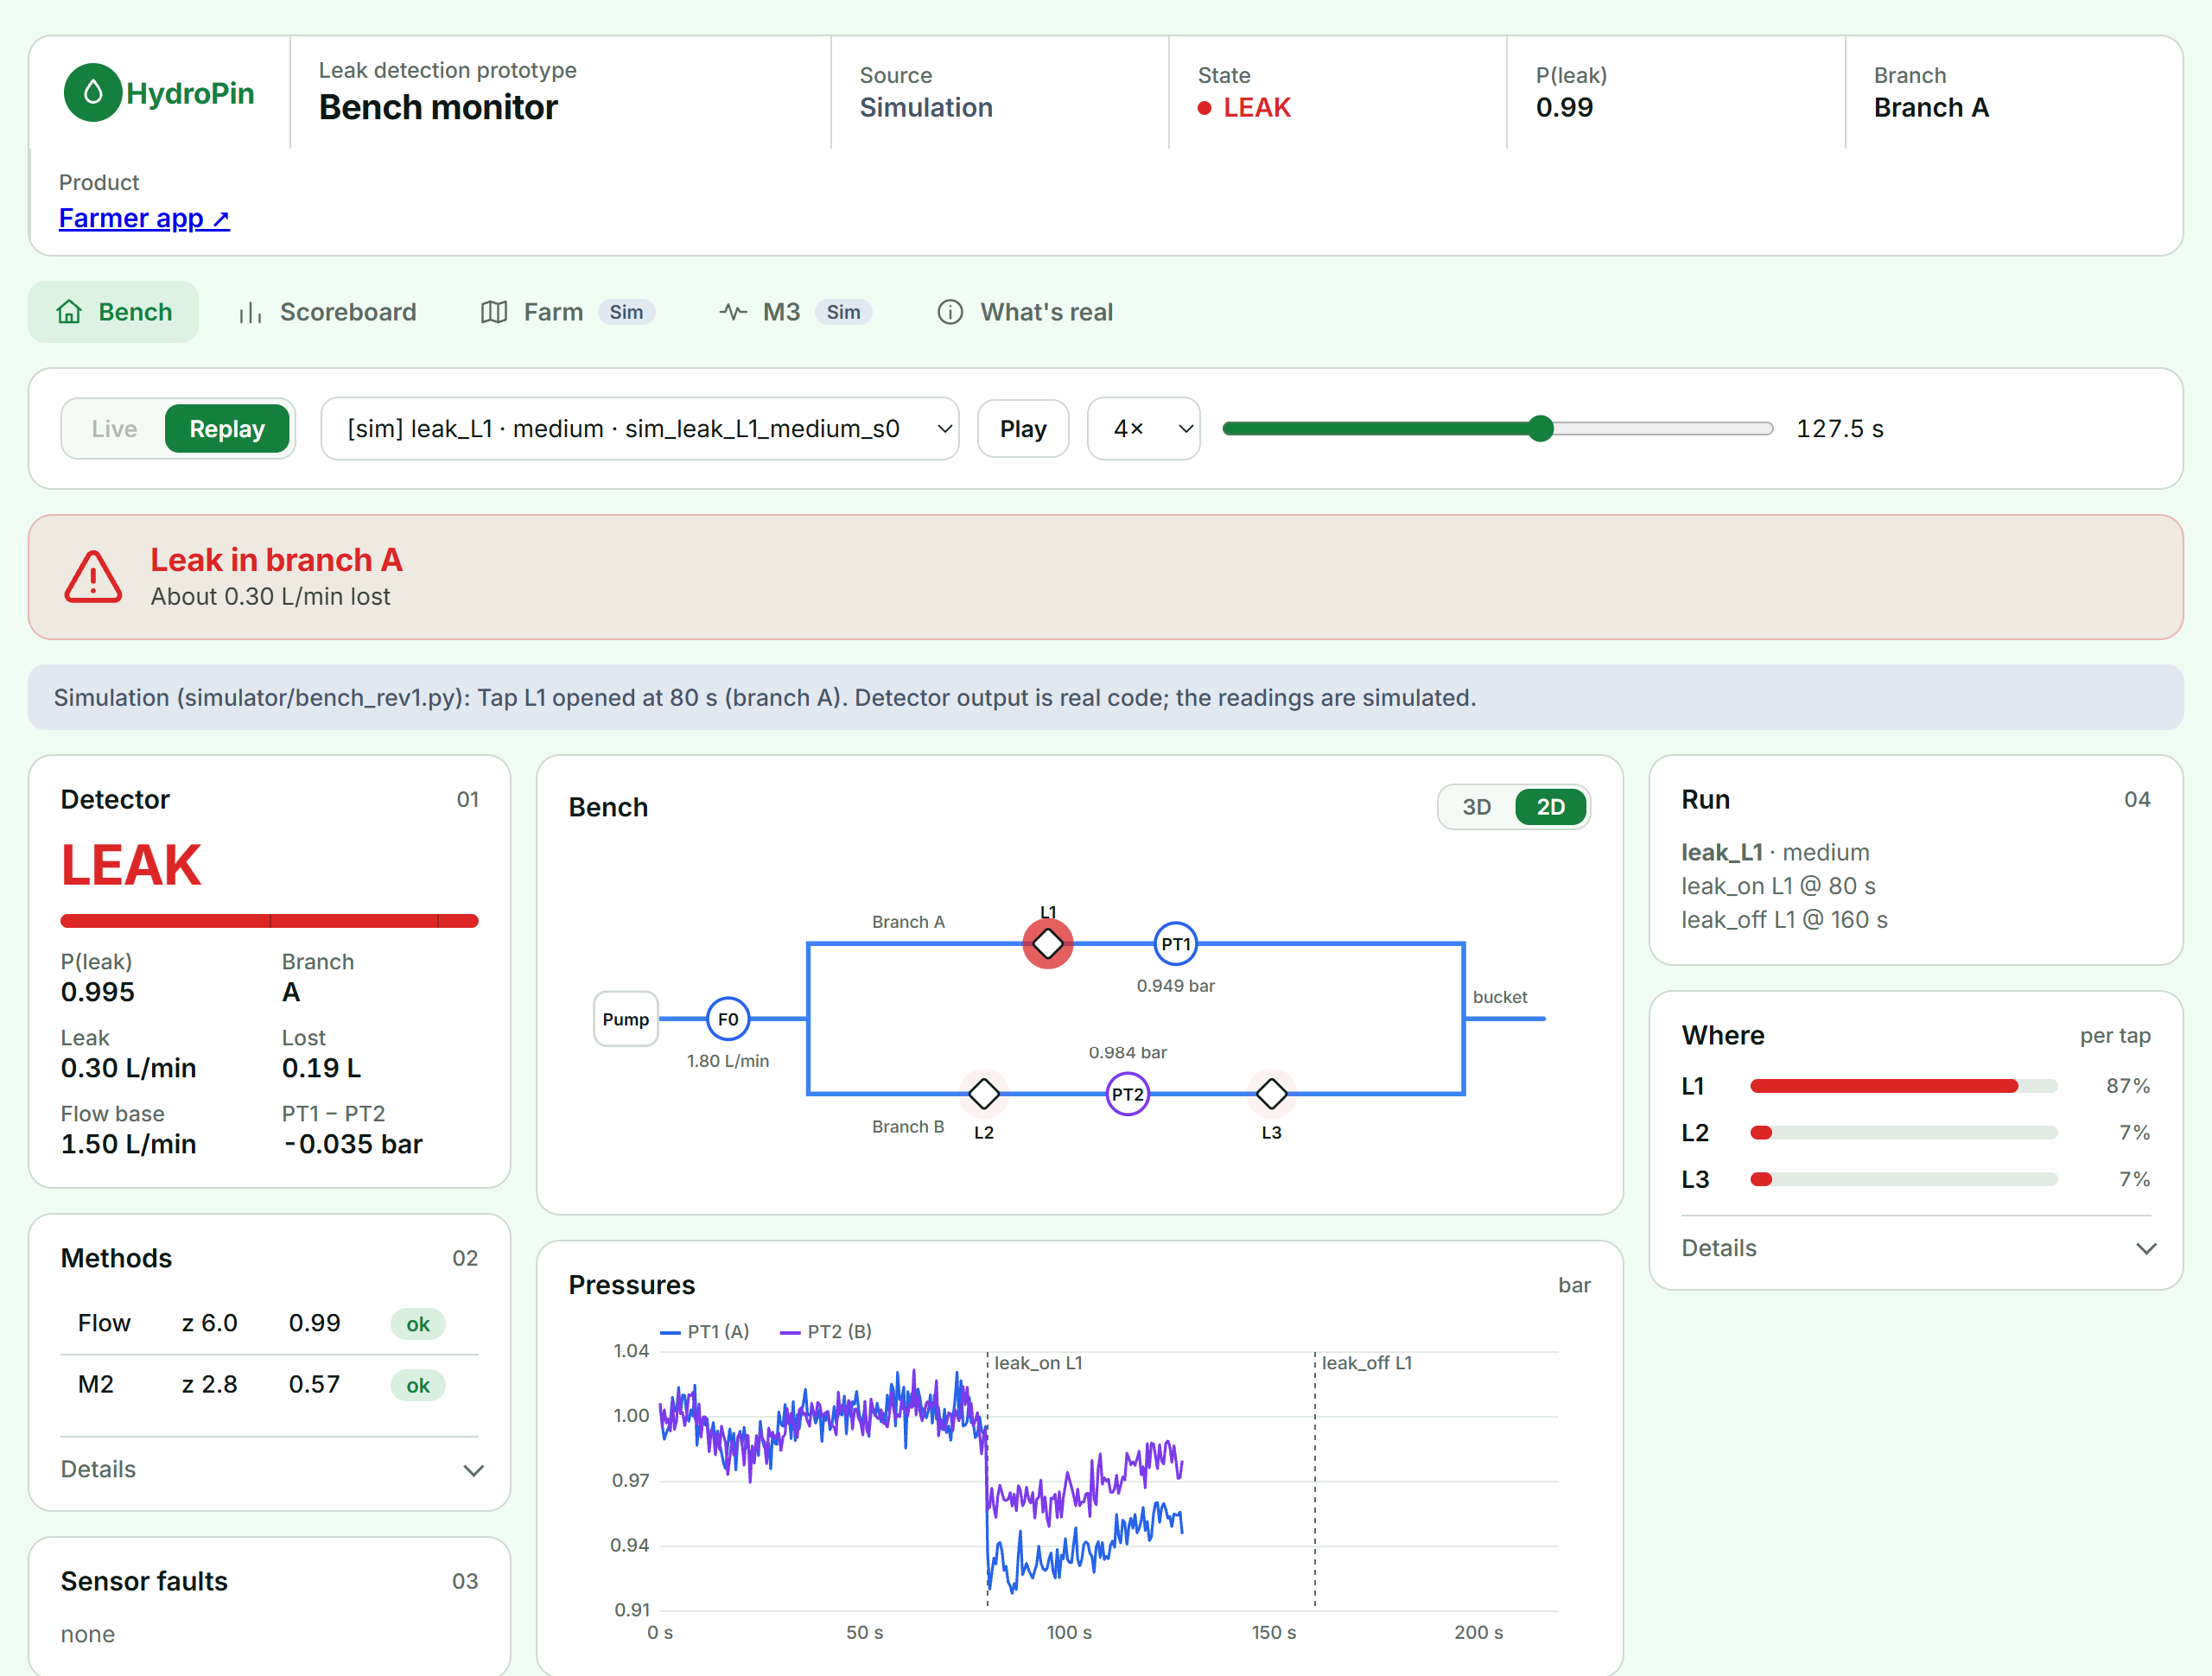
\includegraphics[width=0.92\textwidth]{dash_bench.png}
\caption{Dashboard, Bench tab, replaying a simulated L1 leak opened at 80~s. The alert reads
``Leak in branch~A, about 0.30~L/min lost''; the detector is at \textsc{leak} ($p = 0.995$,
0.19~L lost, L1 at 87\,\%), and PT1 drops about twice as much as PT2. A second banner states that
the readings are simulated and the detector output is the real code. The bench drawing also has a
3D view; below this view are the flow and $P(\mathrm{leak})$ charts.}
\label{fig:dashbench}
\end{figure*}

\begin{figure}[t]
\centering
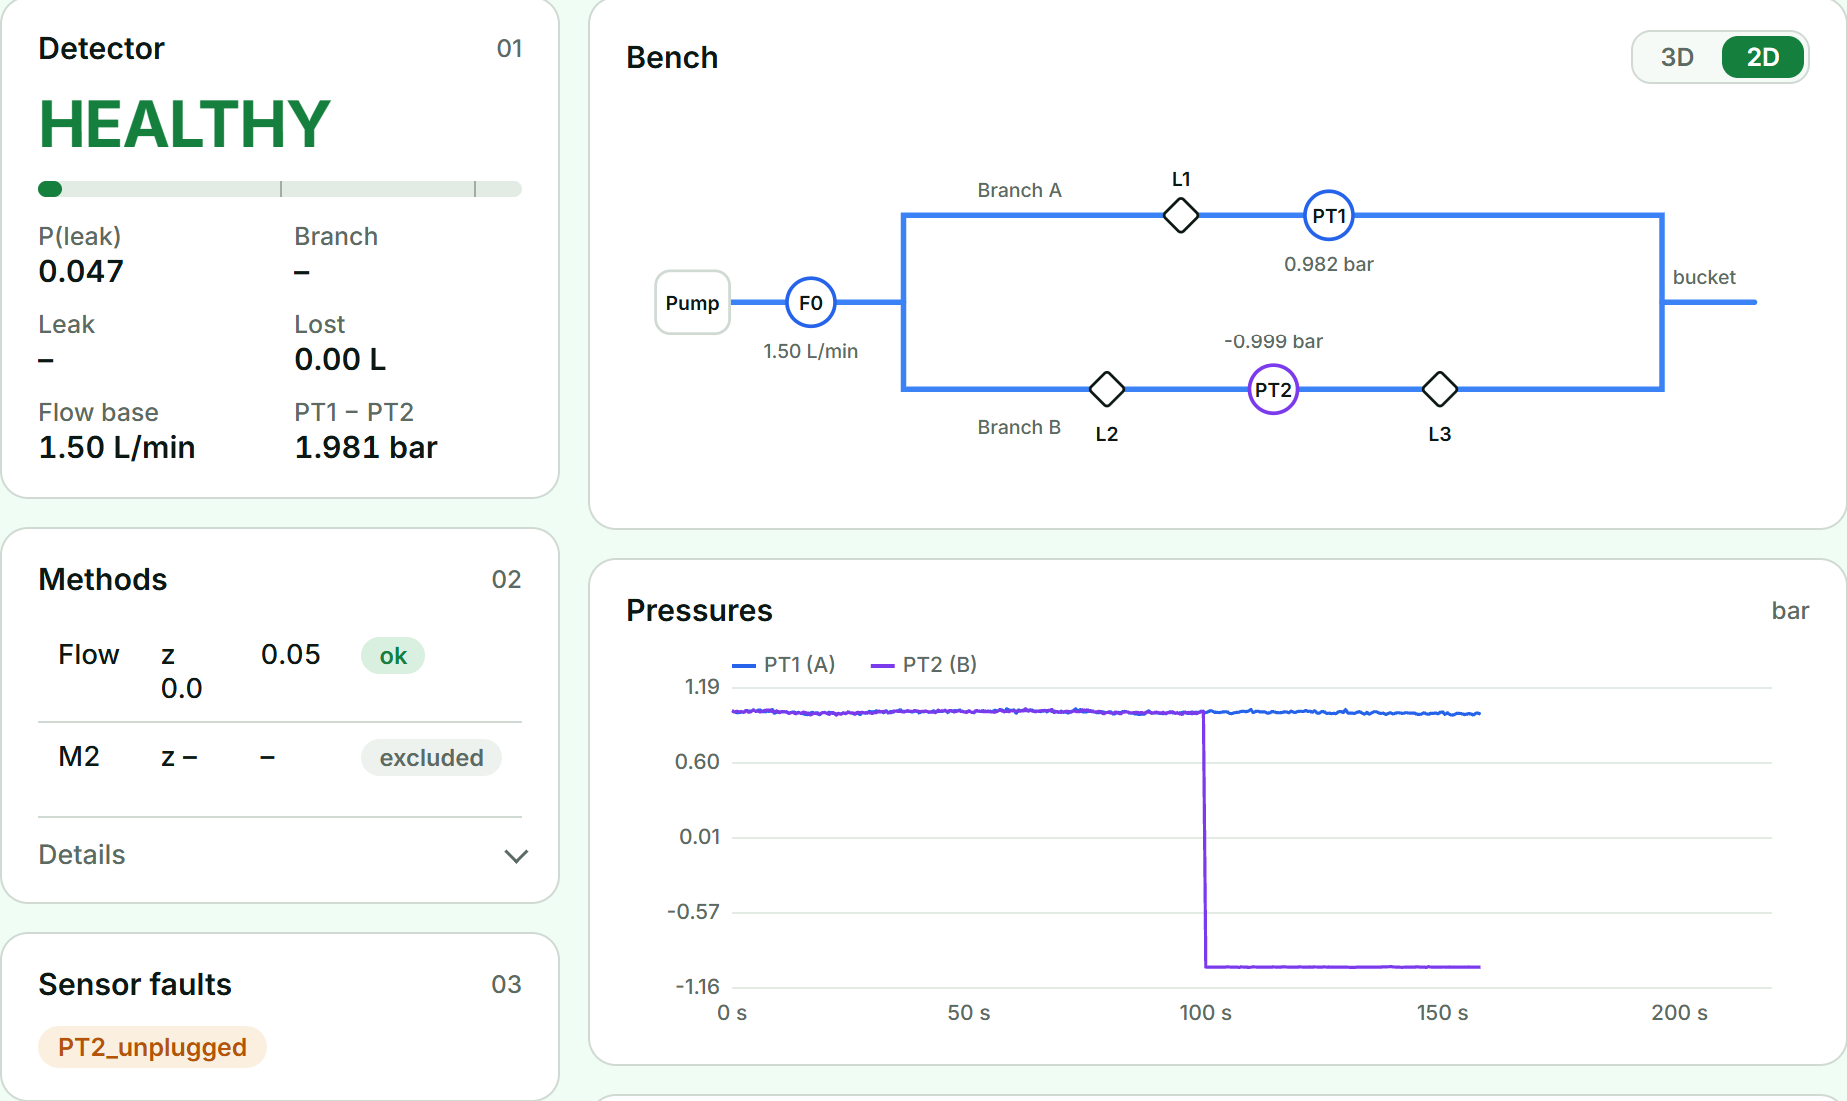
\includegraphics[width=\columnwidth]{dash_fault.png}
\caption{PT2 unplugged at 100~s (simulated). The quality gate raises \texttt{PT2\_unplugged},
excludes M2, and the state stays \textsc{healthy}: a sensor fault, not a leak.}
\label{fig:fault}
\end{figure}

% =====================================================================
\section{Scaling to a Farm (Simulation)}
\label{sec:farm}
\subsection{Virtual farm and leak dataset}
We built a WNTR (EPANET) model~\cite{klise2017} of a plausible Tunisian drip farm
(Fig.~\ref{fig:farm}). All parameters are assumptions, listed in the repository:
\begin{itemize}
\item 50~ha, 700$\times$715~m, six 8.3~ha sectors, two open at a time (three irrigation shifts);
\item a 3-point pump curve (70~L/s at 30~m);
\item a PVC~250 main, PVC~160/PE~125 sub-mains, Hazen--Williams $C = 140$--145;
\item pressure-dependent demand (12~m required at the manifolds) and a gentle slope;
\item 16 realistic sensor spots: pump outlet, main valve boxes, sector heads upstream of the
  valves, sub-main ends.
\end{itemize}

The dataset holds 2,070 steady-state leak scenarios: every pressurised junction and pipe
midpoint (23 sites per shift) $\times$ leaks of 1, 3 and 10\,\% of the open-sector flow
$\times$ 10 perturbed versions of the farm per shift. Each version draws roughness ($\pm$5\,\%),
elevations ($\sigma = 0.5$~m) and emitter clogging (0.8--1.0) at random. The pressure signature
$\Delta P(i,s)$ is the leak pressure minus the healthy pressure \emph{in the same version}.

The simulation confirms the key physics: a 1\,\% leak lowers every pressure by about 20~mbar,
and only the residual differences point to the leak. Sensor noise is $\sigma = 10$~mbar for now.
\TODO{replace by the measured bench $\sigma$ and re-run.}

\begin{figure}[t]
\centering
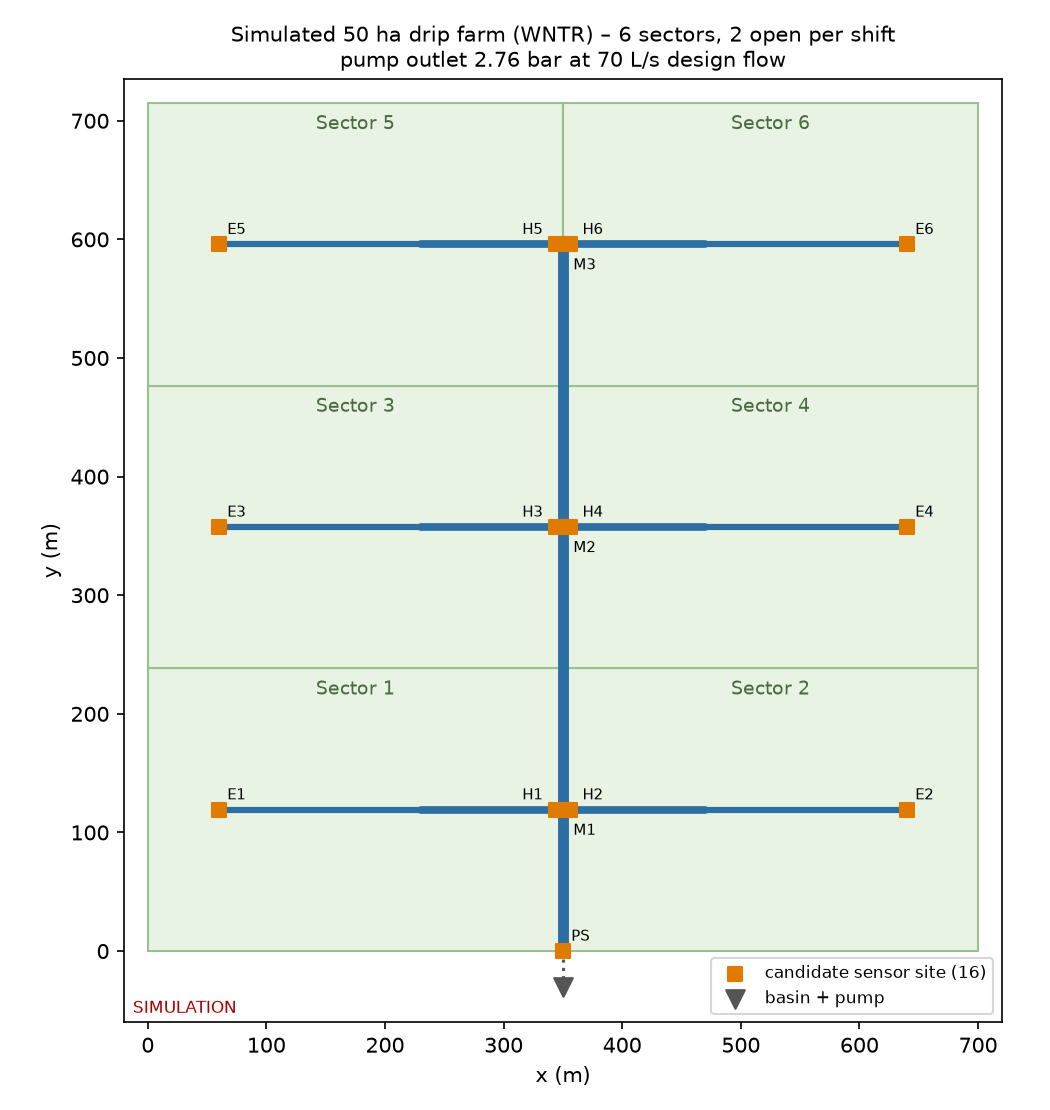
\includegraphics[width=0.86\columnwidth]{farm_layout.png}
\caption{Virtual 50~ha drip farm (\SIM). Orange: the 16 candidate sensor sites.}
\label{fig:farm}
\end{figure}

\subsection{Sensor placement and kit cost}
This follows the blueprint's cost-control algorithm.
\begin{itemize}
\item A set of sensors \emph{detects} leak $s$ if $\max_i |\Delta P(i,s)| > k\sigma$ ($k = 3$).
\item It \emph{isolates} the leak if, once the common mode is removed, the sensor with the
  largest extra drop lies on the leak's branch (main pipe or sector). A sensor in a closed
  sector reads the main pipe and is counted as a main-pipe sensor.
\item For $N = 1$--10 sensors, a nested greedy pick is refined by swaps and a genetic algorithm
  (fixed seed).
\item Each chosen set is re-tested on 10 further perturbed farms (1,380 new simulations).
\end{itemize}
Fig.~\ref{fig:placement} shows the trade-off:
\begin{itemize}
\item one sensor already detects every 3\,\% and 10\,\% leak;
\item isolation grows with the kit: 72\,\% of 3\,\% leaks with 6 nodes (1,752~DT), 83\,\% with 9
  (2,628~DT), and it holds on the perturbed farms;
\item 1\,\% leaks remain at the noise level.
\end{itemize}
No layout reaches 90\,\% isolation, because a leak on the main next to a sector head looks like
a leak just inside that sector. The unit cost of 292~DT (sensor node and tapping point) is an
assumption until the bill of materials is confirmed.

\begin{figure}[t]
\centering
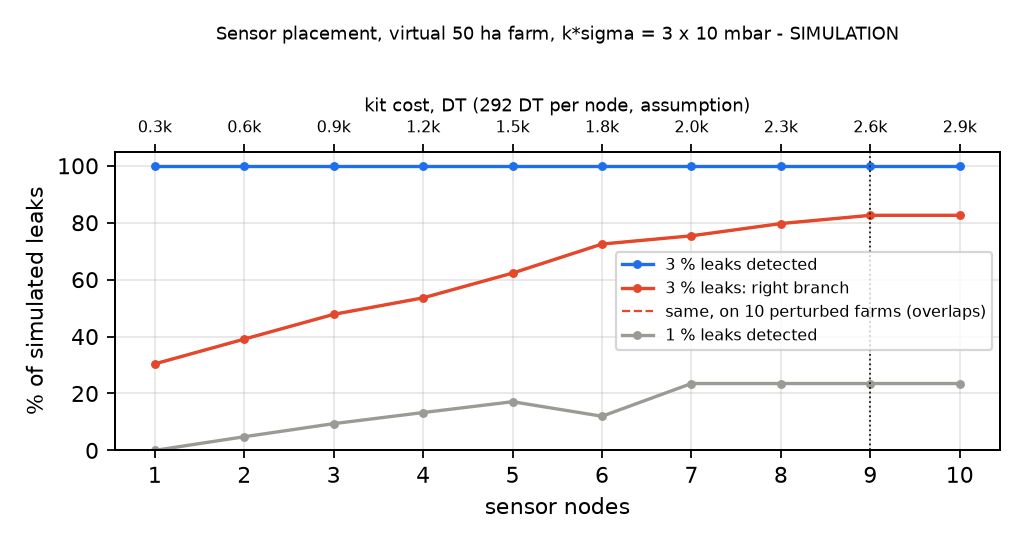
\includegraphics[width=\columnwidth]{farm_placement.png}
\caption{Sensor placement on the virtual farm (\SIM): detection and isolation of 3\,\% leaks vs
number of sensors and kit cost. Dashed: the same sets on 10 perturbed farms (overlapping).}
\label{fig:placement}
\end{figure}

\subsection{Pipe-level localisation: M2, M1 and fusion}
\emph{M2 on the farm} removes the common mode from the residual at the chosen sensors and
compares the remaining pattern $\mathbf D$ with a fingerprint $\mathbf u_s$ learned per leak
site:
\begin{equation}
\log p(s \mid \mathbf D) = \frac{\max(0,\,\mathbf D^\top \mathbf u_s)^2}{2\sigma_{\mathrm{eff}}^2} + \mathrm{const}.
\end{equation}
\emph{M1} is a three-layer graph convolutional network~\cite{kipf2017} on the pipe graph,
$H^{(l+1)} = \mathrm{ReLU}(\hat A H^{(l)} W^{(l)})$ with $\hat A = D^{-1/2}(A+I)D^{-1/2}$. Its
node features are the residual at the sensors, a has-sensor flag, the sector-open flag and the
elevation. A shared head scores junction and pipe sites. The \emph{fusion} is the normalised
product of the two maps.

Both methods are trained on farm versions 0--6 and scored only on versions 7--9.
Table~\ref{tab:farm} uses 1-minute averaged residuals (an assumption: white noise). With 10
sensors the fusion names the exact leaking pipe for half of the leaks and the right branch for
two thirds. From single readings the scores drop (M2: 43\,\% right branch with 6 sensors).

\begin{table}[t]
\caption{Farm localisation on unseen farm versions, 3--10\,\% leaks (\SIM)}
\label{tab:farm}
\centering
\footnotesize
\begin{tabular}{@{}llccc@{}}
\toprule
Sensors & Method & Right branch & Pipe $\pm$1 hop & Exact pipe\\
\midrule
\multirow{3}{*}{6} & M2 & 57\,\% & 43\,\% & 26\,\%\\
 & M1 (GCN) & 60\,\% & 42\,\% & 23\,\%\\
 & Fused & 60\,\% & 47\,\% & 30\,\%\\
\midrule
\multirow{3}{*}{10} & M2 & 64\,\% & 54\,\% & 43\,\%\\
 & M1 (GCN) & 68\,\% & 61\,\% & 37\,\%\\
 & Fused & 67\,\% & 60\,\% & 50\,\%\\
\bottomrule
\end{tabular}
\end{table}

\subsection{Drone confirmation (rule-based)}
The drone is optional and rule-based:
\begin{enumerate}
\item take the pipes holding $\geq$90\,\% of the fused probability;
\item place waypoints every 10~m along them, at 30~m altitude;
\item fly from the pump station in nearest-neighbour order, at 8~m/s with a 10~s hover per pipe;
\item take off at sunrise (07:07 on 27~Nov), when the thermal contrast of wet soil is best.
\end{enumerate}
On the ten showcase leaks with six sensors, the leaking pipe lies on the route in 8~cases, and a
median flight lasts 3.4~min. Fig.~\ref{fig:dashfarm} shows the Farm tab. Real flights through a
vendor SDK or MAVLink, and permits, are next steps.

\begin{figure*}[t]
\centering
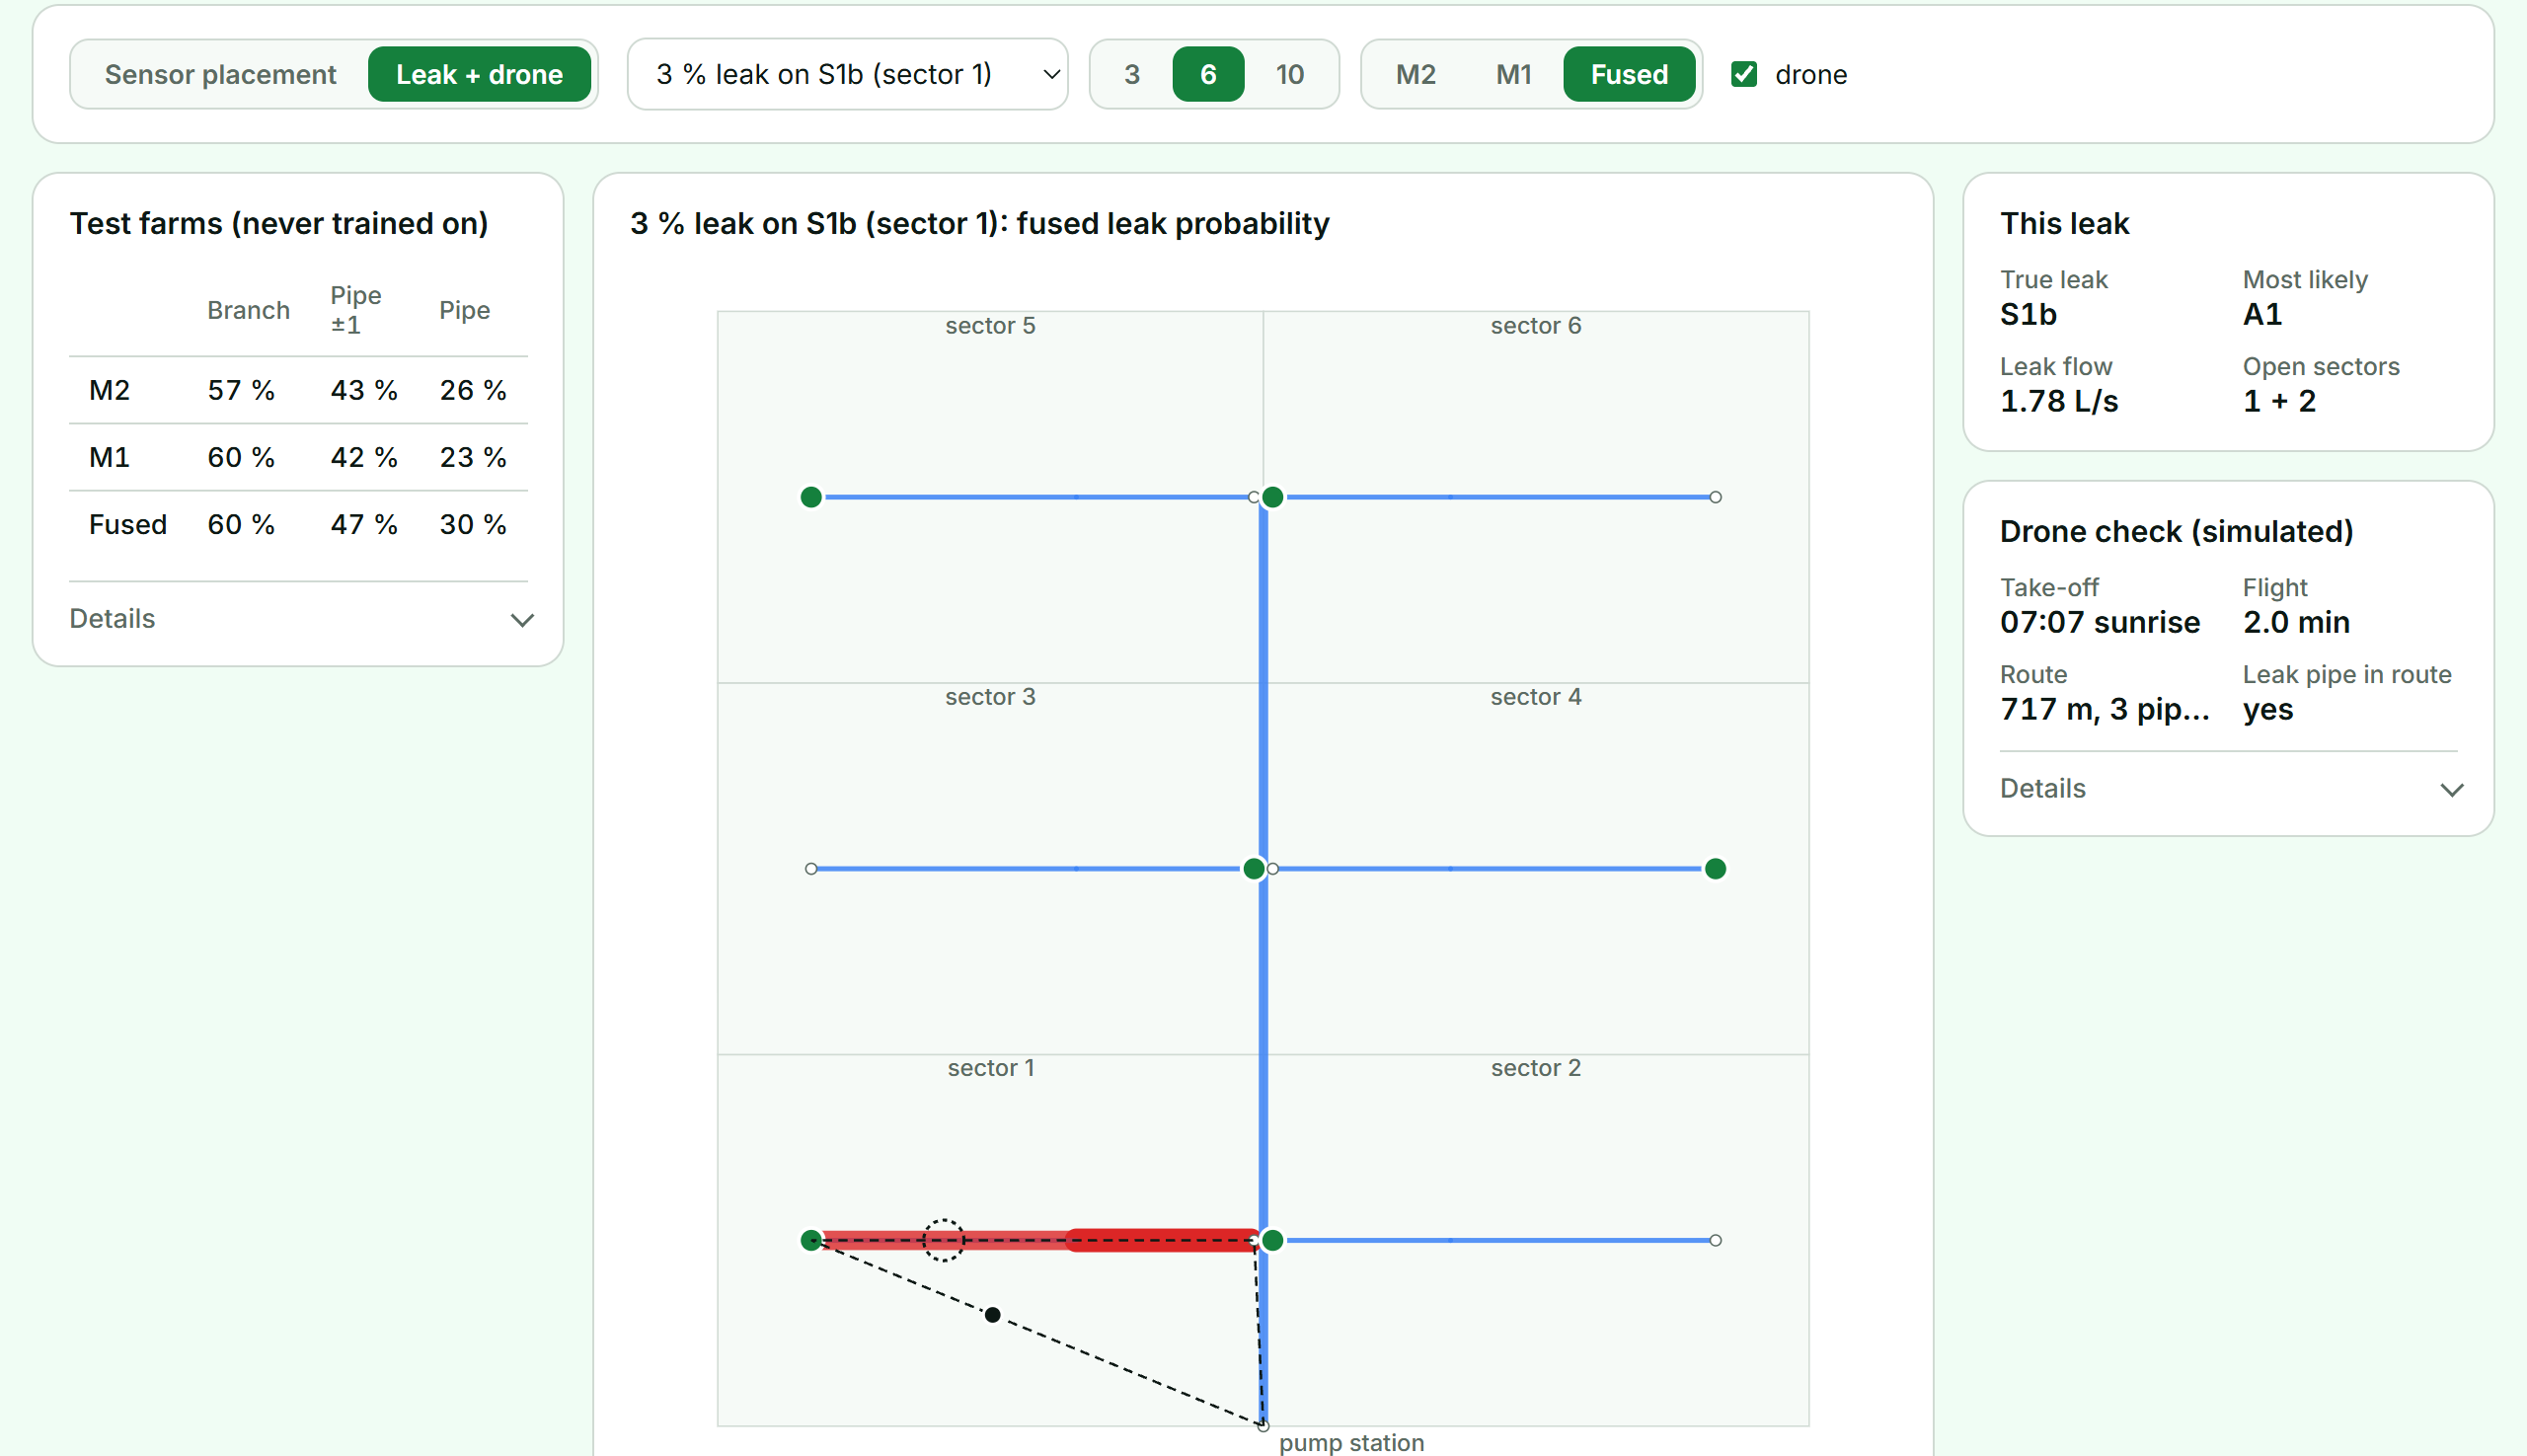
\includegraphics[width=0.92\textwidth]{dash_farm.png}
\caption{Dashboard, Farm tab (\SIM): a 3\,\% leak on sub-main S1b with six sensors (green
dots). Red: fused leak probability per pipe. Dashed ring: true leak. Black dashed line: the
sunrise drone route (717~m, 2.0~min), which covers the leaking pipe. Left: scores on unseen farm
versions.}
\label{fig:dashfarm}
\end{figure*}

% =====================================================================
\section{M3: Pressure-Wave Localisation (Simulation)}
\label{sec:m3}
The bench cannot sample at kHz rates or close a valve in 25~ms, so M3 is developed in simulation
(team decision). The setup is a 150~m PE pipe (50~mm, wave speed $a = 350$~m/s) with a reservoir
upstream and a fast valve and pressure sensor downstream. The sensor records 2~kHz. A leak
orifice follows $Q_L = C_d A_L \sqrt{2gH}$.

The method of characteristics~\cite{wylie1993,chaudhry2014} with Courant number~1 solves
\begin{equation}
H_P = \tfrac12\,(C_P + C_M),\qquad Q_P = \frac{C_P - C_M}{2B},\qquad B = \frac{a}{gA},
\end{equation}
with steady friction in $C_P, C_M$ and quadratic boundary conditions at the valve and at the leak.

\textbf{Validation came first} (Fig.~\ref{fig:m3val}):
\begin{itemize}
\item the Joukowsky jump $a\Delta V/g = 17.845$~m and the period $4L/a = 1.714$~s are reproduced
  exactly;
\item grid convergence and leak mass balance pass;
\item the echo of a 5\,\% leak at 100~m is located within 0.25~m.
\end{itemize}

Four locators run on the same recordings:
\begin{enumerate}
\item echo timing, $x = a\,t_{\mathrm{echo}}/2$;
\item time reversal~\cite{waqar2023}: the leak-induced part of the trace is time-reversed and
  injected into the intact-pipe model, and the energy $E(x) = \int h^2\,dt$ focuses at the leak;
\item matched-field processing~\cite{wang2020};
\item a 1D CNN in the spirit of~\cite{waqar2025}, trained on 9,000 simulated pipes with random
  leak position and size, wave speed, friction and wall creep.
\end{enumerate}
Table~\ref{tab:m3} and Fig.~\ref{fig:m3} summarise the accuracy:
\begin{itemize}
\item with a well-known pipe, time reversal and matched-field reach centimetres to a few
  decimetres;
\item a 5--10\,\% wave-speed error moves them by metres, while the CNN stays below 1~m;
\item time reversal with the wave speed identified from the recording itself stays at 0.27~m
  for every wave-speed error.
\end{itemize}
PE wall creep weakens the echoes and is modelled.

\begin{figure}[t]
\centering
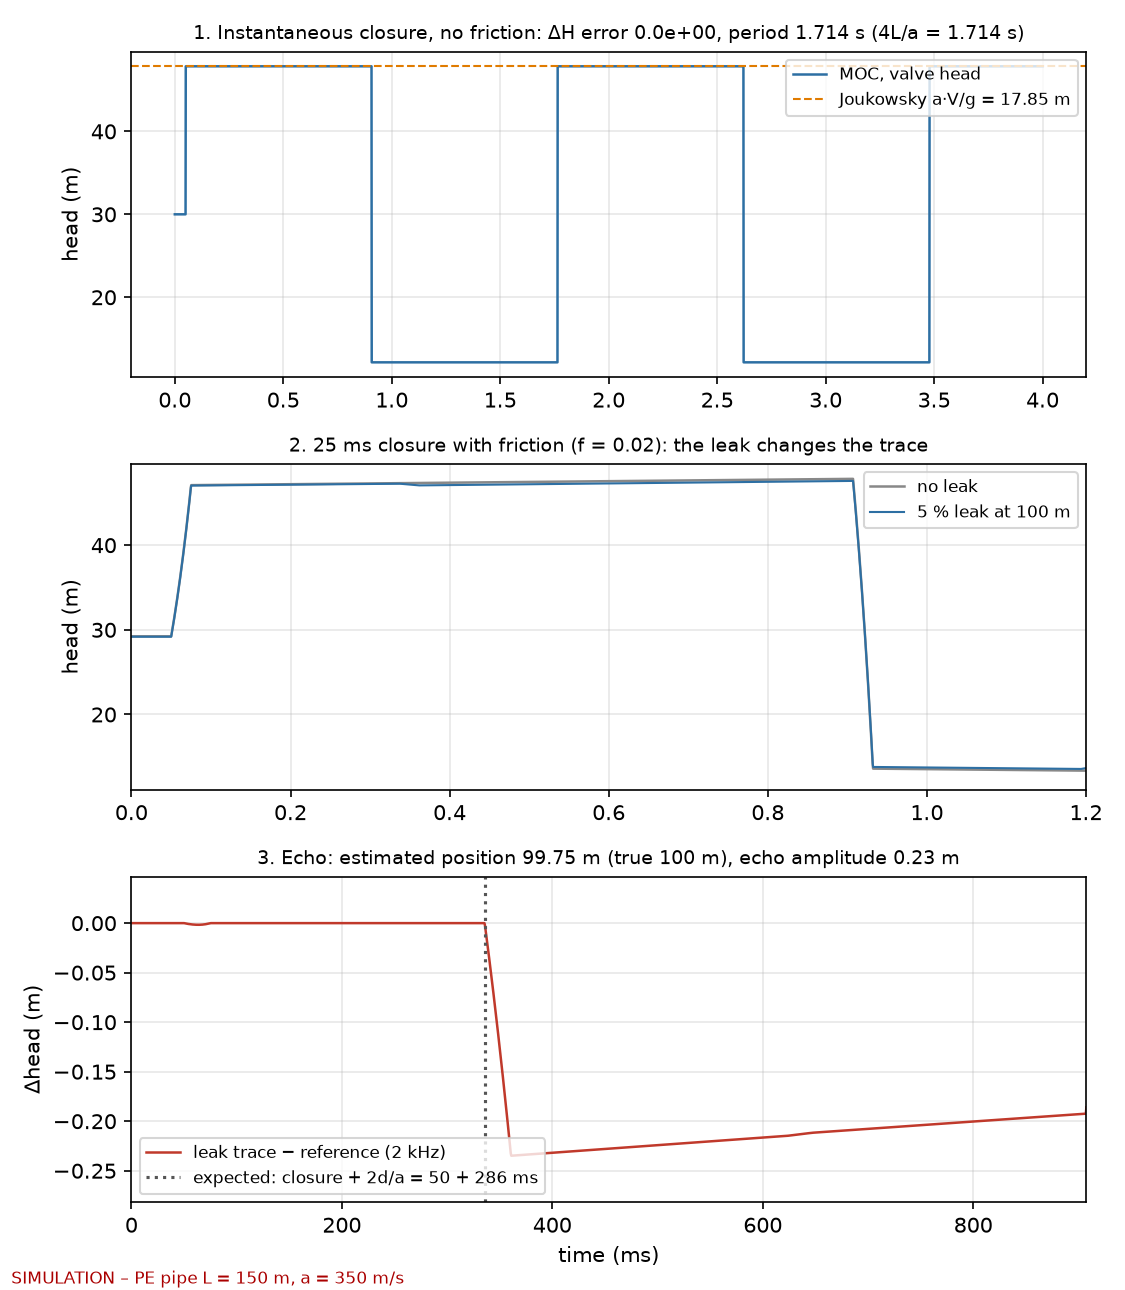
\includegraphics[width=\columnwidth]{m3_validation.png}
\caption{M3 solver validation (\SIM): Joukowsky plateau and $4L/a$ period, effect of a leak on a
25~ms closure, and the leak echo located at 99.75~m (true 100~m).}
\label{fig:m3val}
\end{figure}

\begin{table}[t]
\caption{M3 mean absolute error over 18 test traces (\SIM, m)}
\label{tab:m3}
\centering
\footnotesize
\begin{tabular}{@{}lccccc@{}}
\toprule
Condition & TR & MFP & Echo & CNN & CNN cal.\\
\midrule
noise $\sigma = 0.05$ m & 0.27 & 0.06 & 0.82 & 0.97 & 0.77\\
noise $\sigma = 0.2$ m & 8.2 & 8.8 & 34 & 2.8 & 1.9\\
wave speed +5\,\% & 3.1 & 3.2 & 3.7 & 0.92 & 0.72\\
wave speed +10\,\% & 23 & 8.2 & 24 & 0.92 & 0.72\\
\bottomrule
\end{tabular}
\end{table}

\begin{figure*}[t]
\centering
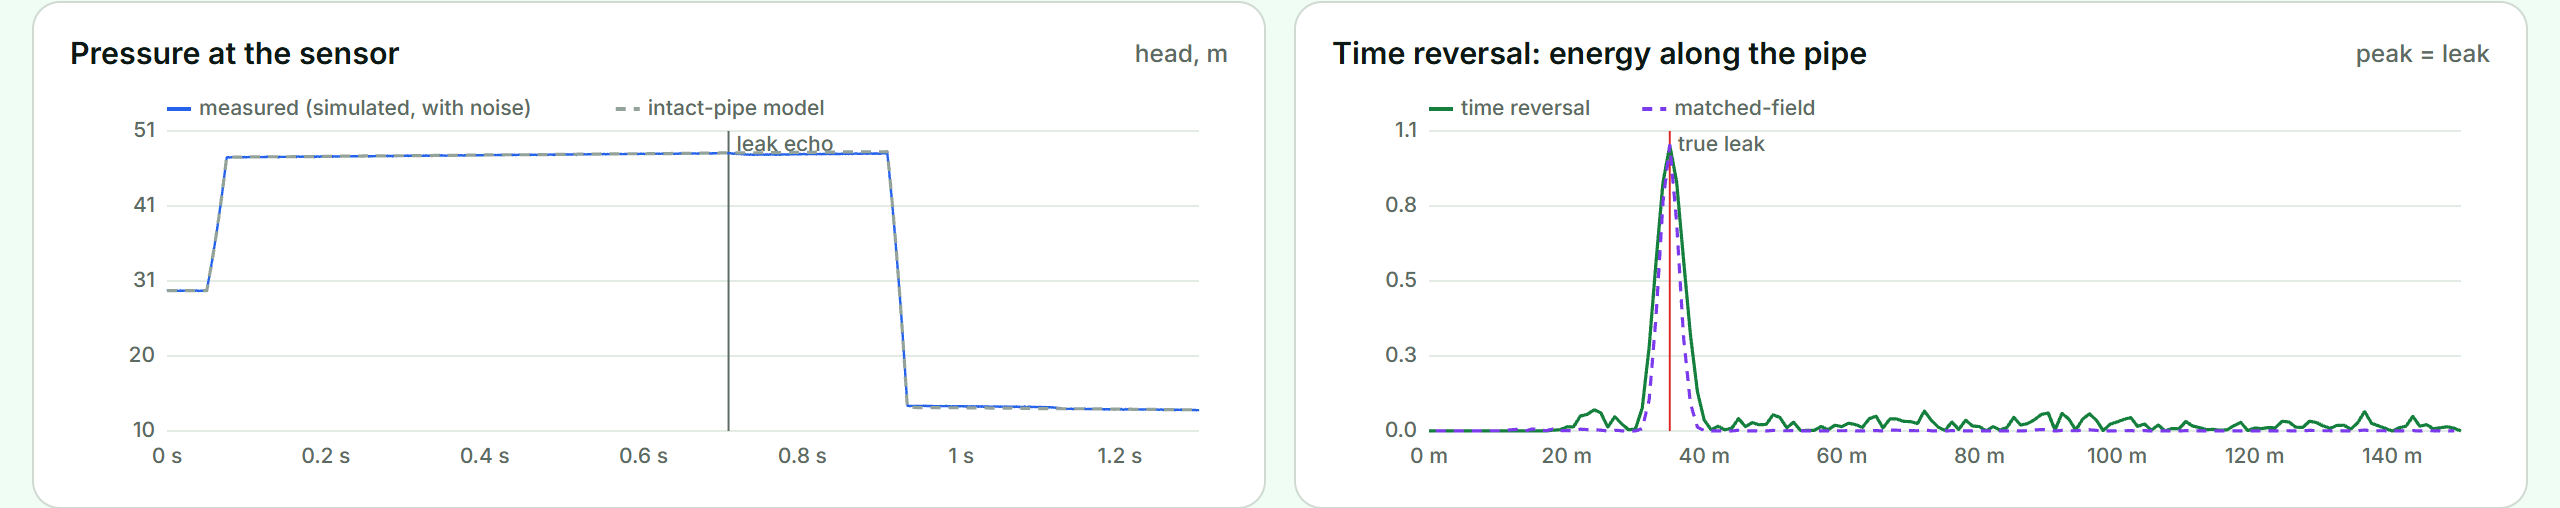
\includegraphics[width=0.92\textwidth]{dash_m3.png}
\caption{Dashboard, M3 tab (\SIM), leak 115~m from the sensor: the valve pressure against the
intact-pipe model, with the leak echo (left); the time-reversal and matched-field energy along the
pipe, peaking at the true leak (right). Errors: TR 0.0~m, MFP 0.0~m, echo 0.85~m, CNN 2.2~m.}
\label{fig:m3}
\end{figure*}

% =====================================================================
\section{Software Platform and Dashboard}
\textbf{Contract.} The frozen message schema, REST API, replay format and dashboard data files
are versioned in the repository. Changes are made only by agreement, with a version bump.

\textbf{Backend.} The MQTT client runs in a background thread and hands frames to the asyncio
loop; WebSocket clients are never touched from the MQTT thread. SQLite stores readings, runs,
events, alerts and processed frames. The REST API offers:
\begin{itemize}
\item the current state and the run controls (start, stop, metadata);
\item ground-truth events (leak on/off, valve change, pump on/off) and re-baselining;
\item CSV export and replay files.
\end{itemize}
Telegram messages (leak, new sensor fault, resolved) are sent in a background thread, so a
network problem never blocks ingestion.

\textbf{Dashboard.} The dashboard is static HTML, CSS and ES modules with plain SVG charts, no
build step and no CDN, and it works at phone width. It has five tabs: Bench (live or replay, with
a 2D drawing and a 3D model of the bench), Scoreboard, Farm, M3 and ``What's real''. A separate
farmer app (French, Arabic, English; installable on a phone) presents the same detector output in
plain words: where the leak is, a route to it, and the water and money saved. The Scoreboard
(Fig.~\ref{fig:score}) reports, for
the fused result and for each method alone:
\begin{itemize}
\item detection rate, right branch and right tap;
\item time to detect and false alarms per hour;
\item a confusion table and the blind test with its misses.
\end{itemize}

\textbf{Campaign tooling.} One command each turns the recorded runs into results:
\begin{itemize}
\item sensor $\sigma$ from the quiet run;
\item a stratified 70/30 train/test split in which blind runs are always test runs, and
  fingerprints and thresholds fitted on training runs only;
\item the scoreboard, report charts and replays, with the headline computed on test runs only.
\end{itemize}
The suite has 397 automated tests (platform, farm/M3 and digital twin).

\begin{figure}[t]
\centering
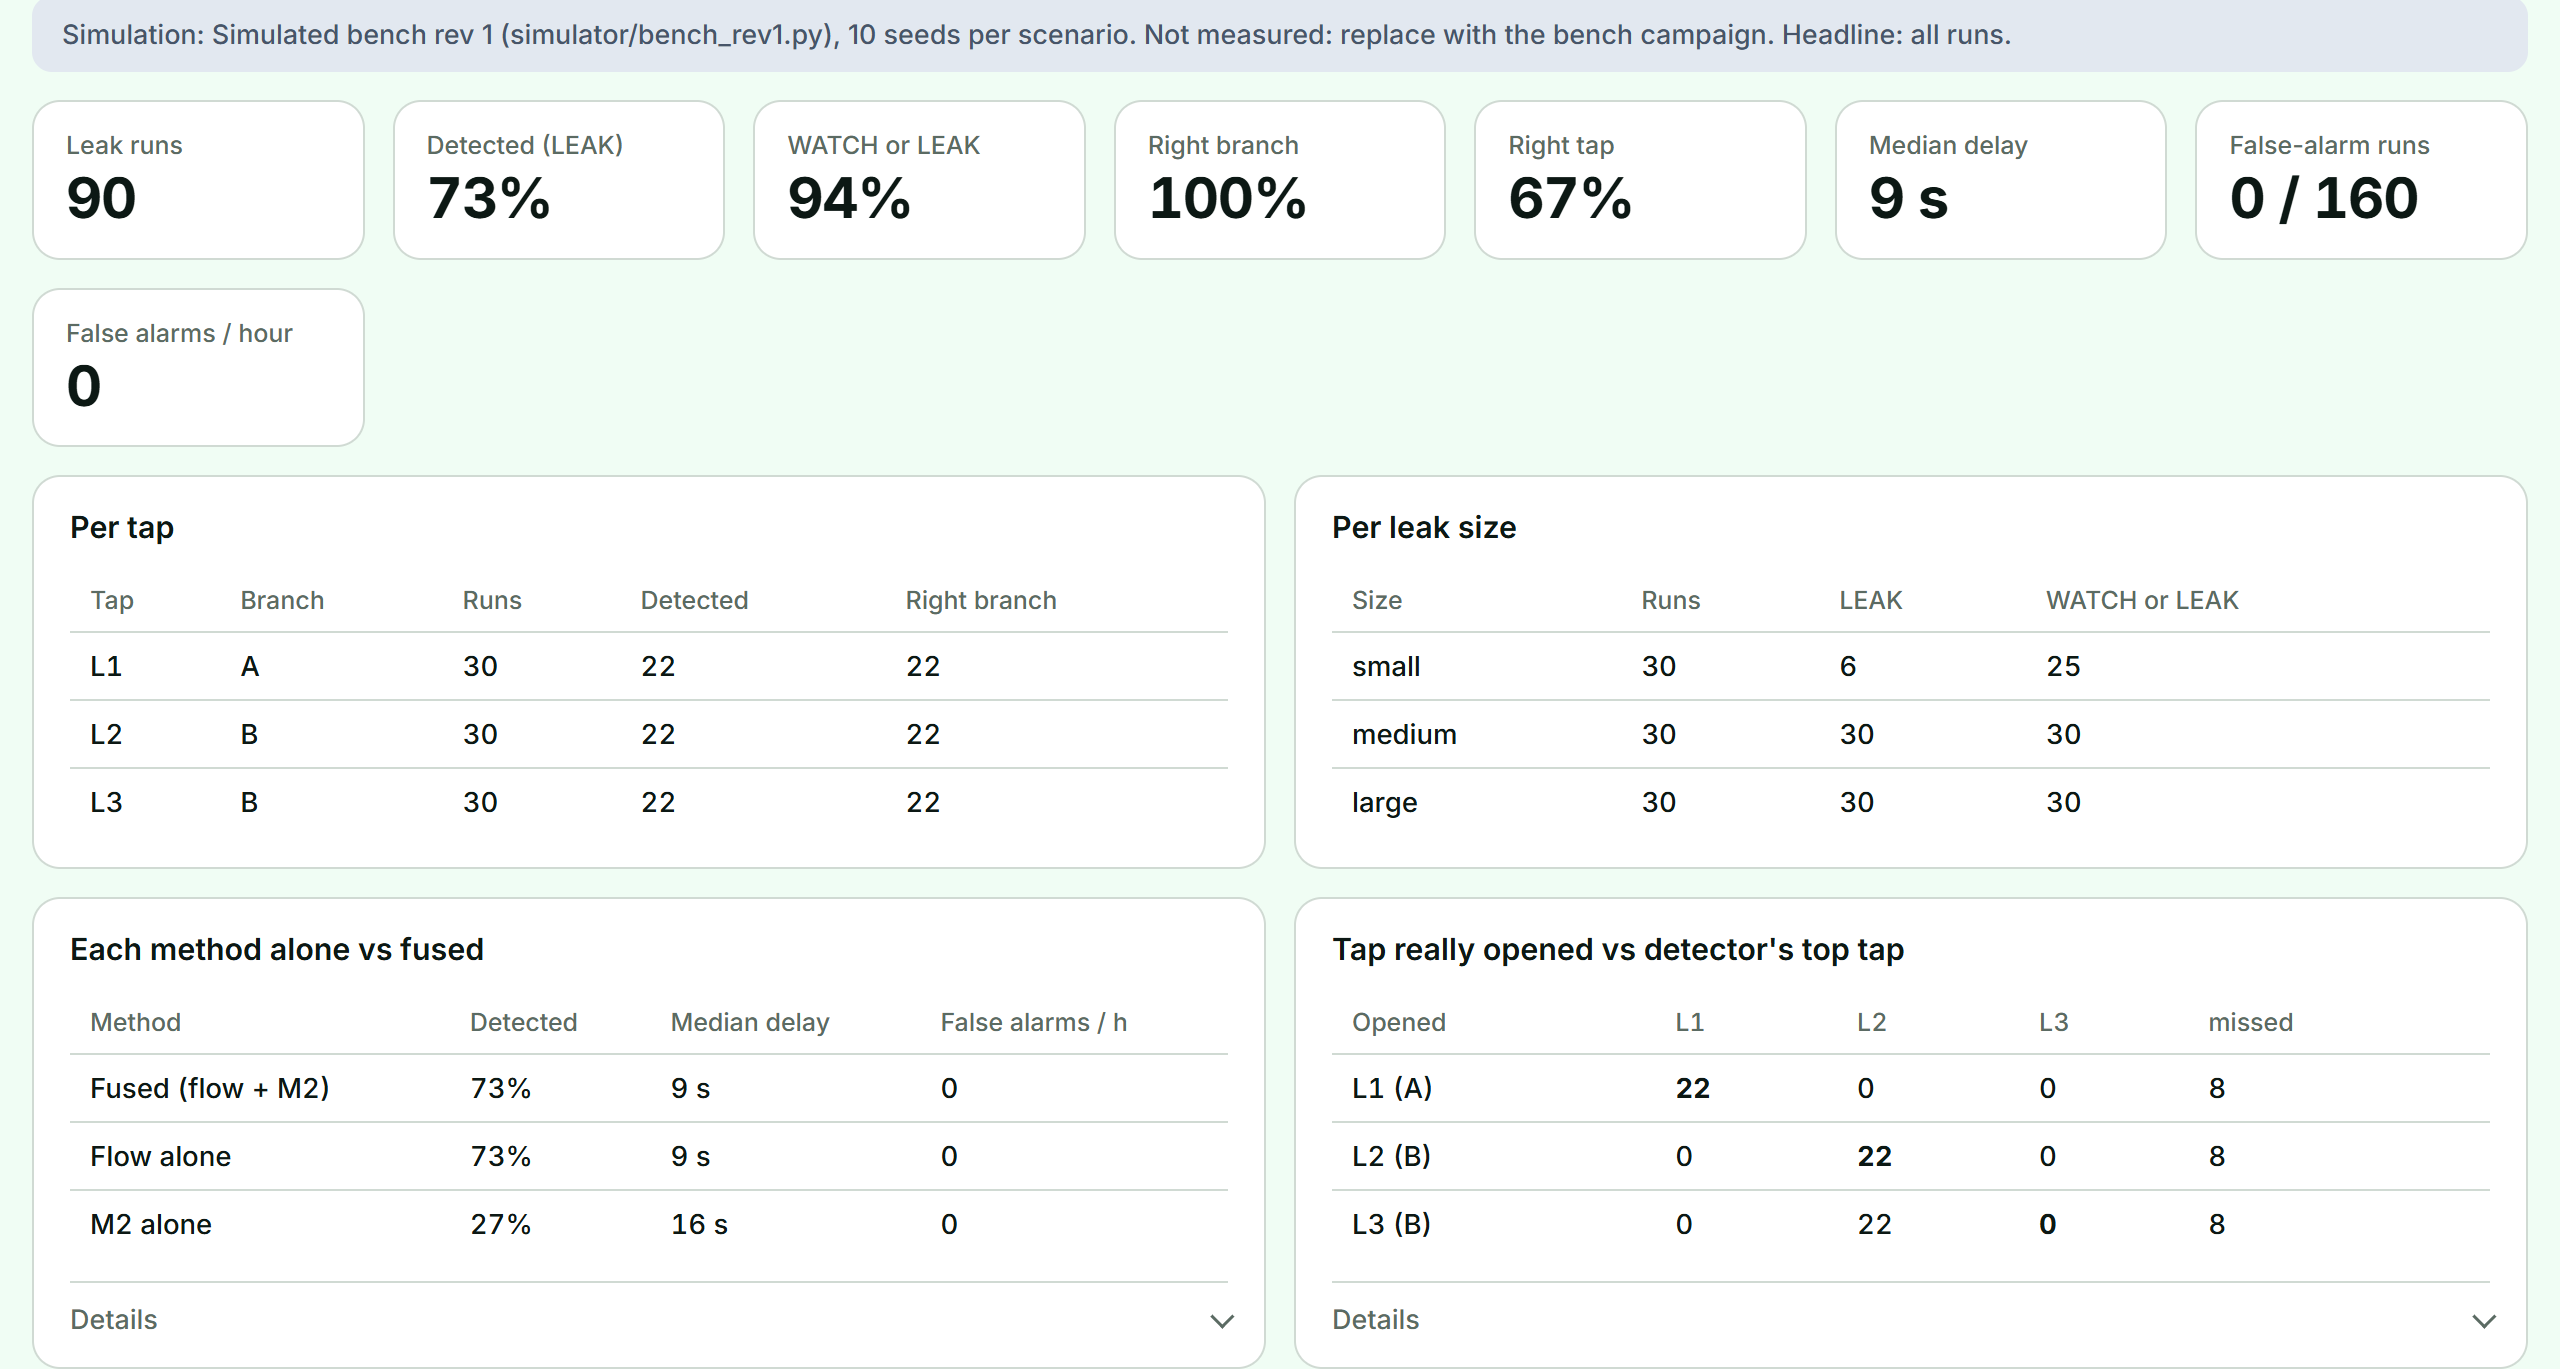
\includegraphics[width=\columnwidth]{dash_scoreboard.png}
\caption{Scoreboard tab, here on the simulated runs. After the campaign it shows the measured
results, with the headline on test runs only.}
\label{fig:score}
\end{figure}

% =====================================================================
\section{Bench Results}
\label{sec:bench}
\TODO{This section is filled from the real campaign. Commands: \texttt{tools.noise},
\texttt{detection.train\_bench}, \texttt{tools.export\_replays --db}, \texttt{detection.report\_charts}.}

\subsection{Bring-up runs, calibration and sensor noise}
Three bring-up runs were recorded on 27~Nov (healthy flow only, no leak), with pressures
recomputed from the raw ADC counts at $\times 3.0$.
\begin{itemize}
\item \textbf{Operating point:} F0 $\approx$ 0.5~L/min, PT2 $\approx$ 0.58~bar,
  PT1 $\approx$ 0.03--0.07~bar.
\item \textbf{Short-term noise} (standard deviation of successive differences$/\sqrt 2$):
  PT2 5--7~mbar, close to the 6~mbar assumed in the simulator; PT1 10--20~mbar; F0 0.04~L/min.
\item \textbf{Data link:} in the two runs on a stable connection, 91--96\,\% of the 2~Hz frames
  arrived, with no gap longer than 1~s. The first run lost 77\,\% of its frames, mostly in one
  7.5-min WiFi outage during bring-up (the detector reports \textsc{offline} after 3~s without
  data).
\end{itemize}
Two findings matter for the campaign:
\begin{itemize}
\item The real flow is about three times lower than the simulator assumed (0.5 vs 1.5~L/min).
  The flow meter's 0.1~L/min step is then about 20\,\% of the flow, so small leaks will be harder
  than in Table~\ref{tab:simscore}; larger openings are preferred.
\item PT1 sits near the bottom of its 0--6~bar range, where its noise is large compared with the
  signal. \TODO{explain or fix: PT1 tapping point or installation.}
\end{itemize}
\TODO{final $\sigma$ from the 10-min quiet run (\texttt{tools.noise}); flow $K$ from the jug
test; zero offsets.}

\subsection{Staged leak campaign}
\TODO{3 baseline runs; 27 leak runs (L1/L2/L3 $\times$ small/medium/large $\times$ 3, random
order; minimum 12); stress runs (pump off/on, valve change + re-baseline, 10-s WiFi cut). Table:
detection rate, right branch, right tap, median time to detect, false alarms per hour, fused vs
flow vs M2, on test runs only. Figures: time-to-detect histogram, tap confusion matrix, example
run.}

\subsection{Blind test}
\TODO{3--5 runs where a teammate opens a tap the operator does not know; every run listed,
misses included.}

\subsection{Digital twin vs real}
\TODO{twin predictions vs measured pressure drops per tap (\texttt{twin.compare}); expected:
L1 drops PT1 $\approx 2\times$ PT2; L2 and L3 nearly identical.}

% =====================================================================
\section{What Is Real, What Is Simulated}
\begin{table}[t]
\caption{Status of each part of the prototype}
\label{tab:real}
\centering
\footnotesize
\begin{tabular}{@{}p{3.1cm}p{1.6cm}p{2.8cm}@{}}
\toprule
Part & Status & Basis\\
\midrule
Bench readings, detector, alerts & measured & bench rev.~1 \TODO{campaign}\\
Detector validation (Table~\ref{tab:simscore}) & simulation & bench simulator\\
Virtual farm, placement, M1/M2 & simulation & WNTR, unseen farm versions\\
Drone dispatch & simulation & rule-based, no flight\\
M3 pressure waves & simulation & validated MOC solver\\
Field pilot & next step & partner farm\\
\bottomrule
\end{tabular}
\end{table}
Table~\ref{tab:real} summarises what each result rests on. The dashboard carries the same
labels.

% =====================================================================
\section{Conclusion and Next Steps}
HydroPin runs end to end, from a low-cost sensor node to a phone alert, with a detector that
separates sensor faults from leaks and names the leaking branch. At farm scale, simulation shows
the core trade-off: one sensor detects, but locating needs several. Six to nine nodes trace most
leaks to the right branch, and a GNN fused with M2 narrows them to a pipe for a sunrise drone
check. Pressure waves with time reversal locate leaks to under a metre on a simulated pipe and
stay robust when combined with a trained model.

Next steps:
\begin{itemize}
\item the field pilot, with measured noise replacing the 10~mbar assumption;
\item calibrating the farm twin on a real network;
\item a fast valve and a kHz sensor to test M3 in the field;
\item real drone flights.
\end{itemize}

\begin{thebibliography}{00}
\bibitem{klise2017} K.~A. Klise, M.~Bynum, D.~Moriarty, and R.~Murray, ``A software framework for assessing the resilience of drinking water systems to disasters with an example earthquake case study,'' \textit{Environ. Model. Softw.}, vol.~95, pp.~420--431, 2017.
\bibitem{kipf2017} T.~N. Kipf and M.~Welling, ``Semi-supervised classification with graph convolutional networks,'' in \textit{Proc. ICLR}, 2017.
\bibitem{wylie1993} E.~B. Wylie and V.~L. Streeter, \textit{Fluid Transients in Systems}. Englewood Cliffs, NJ, USA: Prentice Hall, 1993.
\bibitem{chaudhry2014} M.~H. Chaudhry, \textit{Applied Hydraulic Transients}, 3rd~ed. New York, NY, USA: Springer, 2014.
\bibitem{waqar2023} M.~Waqar, M.~Louati, and M.~S. Ghidaoui, ``Time-reversal technique for pipeline defect detection,'' \textit{Water Res.}, vol.~243, art.~120375, 2023, doi: 10.1016/j.watres.2023.120375.
\bibitem{wang2020} X.~Wang, M.~Waqar, H.-C. Yan, M.~Louati, M.~S. Ghidaoui, P.~J. Lee, S.~Meniconi, B.~Brunone, and B.~Karney, ``Pipeline leak localization using matched-field processing incorporating prior information of modeling error,'' \textit{Mech. Syst. Signal Process.}, vol.~143, art.~106849, 2020, doi: 10.1016/j.ymssp.2020.106849.
\bibitem{waqar2025} M.~Waqar, A.~M. Memon, M.~Louati, and M.~S. Ghidaoui, ``Pipeline leak detection using hydraulic transients and domain-guided machine learning,'' \textit{Mech. Syst. Signal Process.}, vol.~224, art.~111967, 2025. \TODO{confirm the article number 111967 on ScienceDirect.}
\end{thebibliography}

\end{document}
